\documentclass[noheader]{coursclass}

\usepackage{tcolorbox}

\begin{document}

On présente la preuve suivante d'une propriété de cours :

\begin{propriete}
	Si $X$ et $Y$ sont des évènements, on a
	$$ P(X ∪ Y) = P(X) + P(Y) - P(X ∩ Y)$$
\end{propriete}

\begin{tcolorbox}
	\textbf{\uline{{\large Démonstration :}}} \bigskip

	On note :
	\begin{itemize}
		\item $x_1$ ; ⋯ ; $x_i$ les issues qui sont dans $X$ mais pas dans $Y$ ;
		\item $y_1$ ; ⋯ ; $y_k$ les issues qui sont dans $Y$ mais pas dans $X$ ;
		\item $z_1$ ; ⋯ ; $z_j$ les issues qui sont dans $X$ et dans $Y$.
	\end{itemize}

	On fait un schéma représentant la situation :
	\begin{center}
		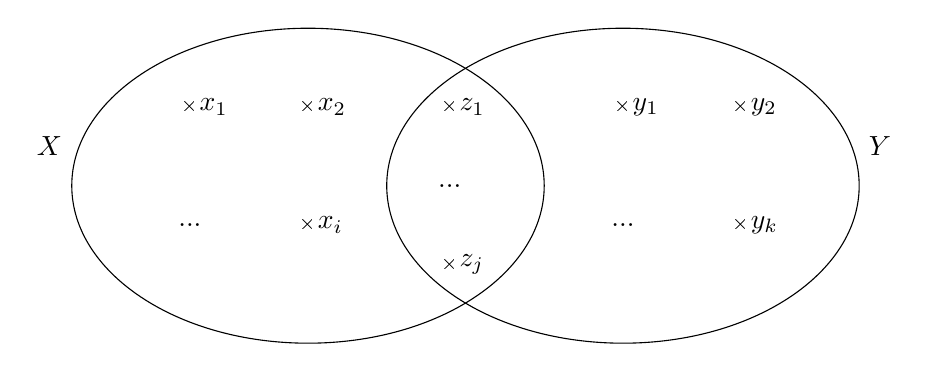
\begin{tikzpicture}
			\draw (-2,0) ellipse (3 and 2); \node[left] at (-5,0.5) {$X$};
			\draw (2,0) ellipse (3 and 2); \node[right] at (5,0.5) {$Y$};

			\node (P) at (-3.5,1) {{\scriptsize ×}}; \node[right] at (P) {$x_1$};
			\node (P) at (-2,1) {{\scriptsize ×}}; \node[right] at (P) {$x_2$};
			\node (P) at (-3.5,-0.5) {$...$};
			\node (P) at (-2,-0.5) {{\scriptsize ×}}; \node[right] at (P) {$x_i$};

			\node (P) at (-0.2,1) {{\scriptsize ×}}; \node[right] at (P) {$z_1$};
			\node (P) at (-0.2,0) {$...$};
			\node (P) at (-0.2,-1) {{\scriptsize ×}}; \node[right] at (P) {$z_j$};

			\node (P) at (2,1) {{\scriptsize ×}}; \node[right] at (P) {$y_1$};
			\node (P) at (3.5,1) {{\scriptsize ×}}; \node[right] at (P) {$y_2$};
			\node (P) at (2,-0.5) {$...$};
			\node (P) at (3.5,-0.5) {{\scriptsize ×}}; \node[right] at (P) {$y_k$};
		\end{tikzpicture}
	\end{center}

	Ainsi on a :

	\begin{center}
		\begin{tabular}{llll}
			             & Uniquement dans $X$       & Uniquement dans $Y$      & Dans $X$ \textbf{ET} dans $Y$ \\ \hline
			             &                           &                          &                               \\
			$P(X) =$     & $P(x_1) + ⋯ + P(x_i)\ + $ &                          & $P(z_1) + ⋯ + P(z_j)$         \\
			$P(Y) =$     &                           & $P(y_1) + ⋯ + P(y_k)\ +$ & $P(z_1) + ⋯ + P(z_j)$         \\
			$P(X ∩ Y) =$ &                           &                          & $P(z_1) + ⋯ + P(z_j)$         \\
			$P(X ∪ Y) =$ & $P(x_1) + ⋯ + P(x_i)\ +$  & $P(y_1) + ⋯ + P(y_k)\ +$ & $P(z_1) + ⋯ + P(z_j)$         \\
		\end{tabular}
	\end{center}

	Et donc :
	\begin{align*}
		P(X) + P(Y) & = P(x_1) + ⋯ + P(x_i) + P(y_1) + ⋯ + P(y_k) + P(z_1) + ⋯ + P(z_j) + P(z_1) + ⋯ + P(z_j) \\
		            & = P(X ∪ Y) + P(X ∩ Y)
	\end{align*}

	Donc $$P(X ∪ Y) = P(X) + P(Y) - P(X ∩ Y)$$
\end{tcolorbox}

Répondre aux questions suivantes, portant sur la démonstration ci-dessus :
\begin{enumerate}
	\item Quelles sont les issues qui appartiennent à $A ∩ B$ ? \correctionOr{$z_1$, ..., $z_j$}{\makebox[6cm]{\dotfill}}
	\item Quelles sont les issues qui appartiennent à $A ∪ B$ ? \correctionOr{$x_1$, $x_2$, ⋯, $x_i$, $y_1$, $y_2$, ⋯, $y_k$, $z_1$, $z_2$, ⋯, $z_j$}{\makebox[6cm]{\dotfill}}
	\item Quand on calcule la somme $P(X) + P(Y)$, quelles sont les issues dont les probabilités sont comptées deux fois ?
\end{enumerate}

\end{document}